\newpage

\chapter{Vibrační podavač s voicecoily firmy \emph{DESSEQ}}
\label{sec::voicecoil_function}

Běžné vibrační podavače generují vibrace pomocí rotačních vibrátorů,
což jsou elektrické motory, na jejichž hřídeli je umístěno nevyvážené závaží.
Při otáčení motoru vznikají oscilace v důsledku tohoto nevyvážení rotačního ústrojí.
U takového typu vibrátoru lze řídit pouze výkon otáčky, což má přímý vliv na frekvenci oscilací.

Motivací pro použití vibračního podavače na principu voicecoilu je možnost širšího řízení,
které zahrnuje nejen frekvenci oscilací, ale i jejich amplitudu, výšku vysunutí jádra voicecoilu a
fázi oscilací mezi jednotlivými voicecoily.
Tento přístup umožňuje mnohem přesnější kontrolu nad rychlostí a směrem pohybu součástek po platě,
zejména při kombinaci s dodatečnou snímaním a vyhodnocováním polohy součástek pomocí obrazu z kamery.
Tímto způsobem lze dosáhnout vyšší přesnosti a efektivity při manipulaci jak s drobnými, tak s velkými součástkami.


\begin{figure}[htbp]
	\centering
	\includegraphics[width=0.95\textwidth]{kapitola6/Figures/vibration_desk.png}
	\caption{Testend vibrační stolice firmy \emph{DESSEQ}}
	\label{fig::vibrator_DESSEQ}
\end{figure}


\section{Snímání polohy}


Pro snímání polohy jádra voicecoilu byla určena metoda snímání změn velikosti
magnetické indukce pomocí senzorů na bázi Hallova jevu.
Optické senzory s dostatečnou datovou prostupností a rozlišením by byly příliš drahé a
kontaktní měření nepřicháyelo v úvahu vzhledem k vibracím a pohybu jádra.
Byly otestovány dvě umístění senzoru.
První umístění bylo na jádře uvnitř voicecoilu a byla měřena magentická indukce jádra.
Druhé umístění bylo na aktuátoru, kde byl měřen magnetický tok přidaného permanentního magnetu.

\subsection{Měření magnetické indukce v jádře voicecoilu}

V prvním prototypu voicecoilu se experimentovalo s umístěním Hallovy sondy na pohyblivém jádře uvnitř voicecoilu.
V tomto případě je magnetická indukce závislá nejen na poloze, ale i na závislosti proudu.
Pro správné určení polohy jádra je nutné znát závislost indukce na proudu a poloze.
Bylo provedeno měření velikosti Hallova napětí při různých proudech a polohách jádra.
Změřená data byla interpolována a následně zdiskretizována do převodní \textit{LUT} tabulky,
která je v tomto případě pole, respektive matice hodnot.
Tato matice hodnot byla nahrána do mikrokontroléru,
který na základě naměřeného Hallova napětí a aktuálního proudu určoval polohu jádra.

\begin{figure}[htbp]
	\centering
	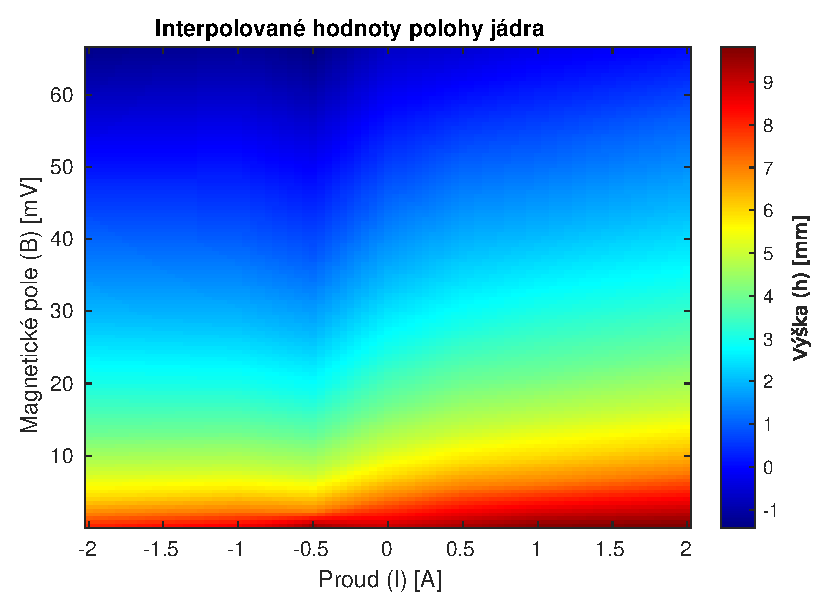
\includegraphics[width=0.9\textwidth]{kapitola6/Figures/hall_on_core_map.eps}
	\caption{Funkce využitá pro určení polohy jádra prvního prototypu}
	\label{fig::hall_oncore_map}
\end{figure}

Ačkoliv tento způsob umístění a řízení polohy jádra voicecoilu fungoval,
jeho největší nevýhodou bylo obtížnější integrace Hallovy sondy do jádra a
také by do útrob jádra musely vést 3 vodiče navíc,
což by ztěžovalo výrobu a montáž.
Bylo tedy přistoupeno k alternativnímu umístění sondy.

\subsection{Měření indukce permanentního magnetu umístěného zvenku voicecoilu}
\label{section::hall_perm_magnet}


V druhém prototypu voicecoilu byl došlo k umístění permanentního neodymového magnetu na statickém magnetickém obvodu jádra.
Hallova sonda byla umístěna na nástavbě připěvněné na pohyblivém jádře.
Motivací k tomuto umístění je nezávislost magnetické indukce na proudu,
což umožňuje přímo měřit polohu jádra bez ohledu na proud procházející cívkou,
ovšem nevýhodou je potřeba přidání permanenetního magnetu.

\begin{figure}[htbp]
	\centering
	\includegraphics[width=0.35\textwidth]{kapitola6/Figures/voicecoil.png}
	\caption{Druhý prototyp voicecoilu. V \textbf{červeném} poli umístěn permanentní magnet,
		v \textbf{modrém} poli pod plastovým krytem umístěna Hallova sonda.}
	\label{fig::voice_coil_second_prototype}
\end{figure}

Pro implementaci do mikrokontroléru bylo změřeno výstupní napětí Hallovy sondy při různých polohách jádra.
Výsledky měření byly interpolovány a zdiskretizovány do převodní \textit{LUT} tabulky,
což je v tomto případě pole, respektive pole, viz \oref{fig::hall_perm_magnet}.
Tato předpočítaná \textit{LUT} tabulka byla nahrána do mikrokontroléru.
Konkrétní implementace ve firmwaru je vidět v \nameref{section::position_regulator}.

\begin{figure}[htbp]
	\centering
	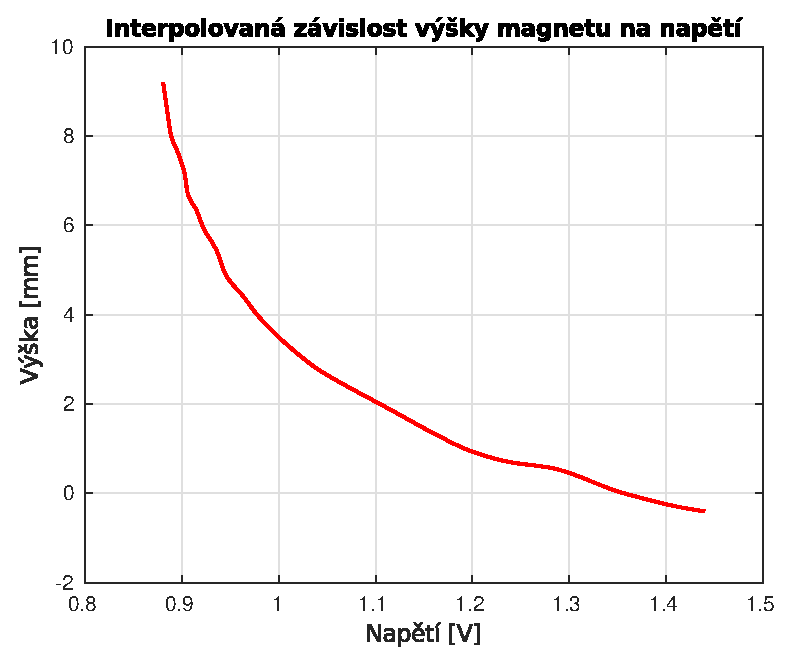
\includegraphics[width=0.9\textwidth]{kapitola6/Figures/hall_perm_magnet2.eps}
	\caption{Funkce využitá pro určení polohy jádra druhého prototypu}
	\label{fig::hall_perm_magnet}
\end{figure}


\subsection{Přesun součástek}

Omtimální nastavení frekvence a amplitudy kmitů, případně fázového posunu mezi jednotlivými voicecoily,
je závislé na velikosti a hmotnosti součástek, které mají být přesouvány.
V ideálním případě by mělo být nastavování těchto parametrů automatizováno,
například pomocí algoritmu, který by na základě snímání polohy součástek skrze kameru,
určil nastavení proudových zdrojů.
Hledání optimálního nastavení pro přesun součástek je však mimo rámec této práce.
